% -----------------------------------------------
% Template for SMC 2019
% adaed from the template for SMC 2018
% -----------------------------------------------

\documentclass{article}
\usepackage{smc2019}
\usepackage{times}
\usepackage{ifpdf}
\usepackage[english]{babel}
\usepackage{cite}

%%%%%%%%%%%%%%%%%%%%%%%% Some useful packages %%%%%%%%%%%%%%%%%%%%%%%%%%%%%%%
%%%%%%%%%%%%%%%%%%%%%%%% See related documentation %%%%%%%%%%%%%%%%%%%%%%%%%%
%\usepackage{amsmath} % popular packages from Am. Math. Soc. Please use the 
%\usepackage{amssymb} % related math environments (split, subequation, cases,
%\usepackage{amsfonts}% multline, etc.)
%\usepackage{bm}      % Bold Math package, defines the command \bf{}
%\usepackage{paralist}% extended list environments
%%subfig.sty is the modern replacement for subfigure.sty. However, subfig.sty 
%%requires and automatically loads caption.sty which overrides class handling 
%%of captions. To prevent this problem, preload caption.sty with caption=false 
%\usepackage[caption=false]{caption}
%\usepackage[font=footnotesize]{subfig}


%user defined variables
\def\papertitle{PHYSICAL MODELS AND REAL-TIME CONTROL WITH THE SENSEL MORPH}
\def\firstauthor{Silvin Willemsen}
\def\secondauthor{Stefan Bilbao}
\def\thirdauthor{Nikolaj
Andersson, Stefania Serafin}

% adds the automatic
% Saves a lot of output space in PDF... after conversion with the distiller
% Delete if you cannot get PS fonts working on your system.

% pdf-tex settings: detect automatically if run by latex or pdflatex
\newif\ifpdf
\ifx\pdfoutput\relax
\else
   \ifcase\pdfoutput
      \pdffalse
   \else
      \pdftrue
\fi

\ifpdf % compiling with pdflatex
  \usepackage[pdftex,
    pdftitle={\papertitle},
    pdfauthor={\firstauthor, \secondauthor, \thirdauthor},
    bookmarksnumbered, % use section numbers with bookmarks
    pdfstartview=XYZ % start with zoom=100% instead of full screen; 
                     % especially useful if working with a big screen :-)
   ]{hyperref}
  %\pdfcompresslevel=9

  \usepackage[pdftex]{graphicx}
  % declare the path(s) where your graphic files are and their extensions so 
  %you won't have to specify these with every instance of \includegraphics
  \graphicspath{{./figures/}}
  \DeclareGraphicsExtensions{.pdf,.jpeg,.png}

  \usepackage[figure,table]{hypcap}

\else % compiling with latex
  \usepackage[dvips,
    bookmarksnumbered, % use section numbers with bookmarks
    pdfstartview=XYZ % start with zoom=100% instead of full screen
  ]{hyperref}  % hyperrefs are active in the pdf file after conversion

  \usepackage[dvips]{epsfig,graphicx}
  % declare the path(s) where your graphic files are and their extensions so 
  %you won't have to specify these with every instance of \includegraphics
  \graphicspath{{./figures/}}
  \DeclareGraphicsExtensions{.eps}

  \usepackage[figure,table]{hypcap}
\fi

%setup the hyperref package - make the links black without a surrounding frame
\hypersetup{
    colorlinks,%
    citecolor=black,%
    filecolor=black,%
    linkcolor=black,%
    urlcolor=black
}


% Title.
% ------
\title{\papertitle}

% Authors
% Please note that submissions are NOT anonymous, therefore 
% authors' names have to be VISIBLE in your manuscript. 
%
% Single address
% To use with only one author or several with the same address
% ---------------
% \twoauthors
%   {\firstauthor} { Multisensory Experience Lab, CREATE,\\ Aalborg University Copenhagen\\
%   Copenhagen, Denmark\\%
%     {\tt \href{mailto:sil@create.aau.dk}{\{sil, nsa, sts\}@create.aau.dk}}}
%     {\secondauthor} { Acoustics and Audio Group \\ University of Edinburgh\\
%     Edinburgh, UK\\
%      {\tt \href{mailto:s.bilbao@ed.ac.uk}{s.bilbao@ed.ac.uk}}}

% Three addresses
% --------------
\threeauthors
  {\firstauthor} { Multisensory Experience Lab, CREATE,\\ Aalborg University Copenhagen\\
  Copenhagen, Denmark\\%
    {\tt \href{mailto:sil@create.aau.dk}{sil@create.aau.dk}}}
  {\secondauthor} { Acoustics and Audio Group \\ University of Edinburgh\\
    Edinburgh, UK\\
     {\tt \href{mailto:s.bilbao@ed.ac.uk}{s.bilbao@ed.ac.uk}}}
  {\thirdauthor}{ Multisensory Experience Lab, CREATE,\\ Aalborg University Copenhagen\\
  Copenhagen, Denmark\\%
    {\tt \href{mailto:sts@create.aau.dk}{\{nsa, sts\}@create.aau.dk}}}
    % {\fourthauthor} { Affiliation4 \\ %
    %  {\tt \href{mailto:author3@smcnetwork.org}{author3@smcnetwork.org}}}

% ***************************************** the document starts here ***************
\begin{document}
%
\capstartfalse
\maketitle
\capstarttrue
%
\begin{abstract}
In this demonstration we present novel physical models controlled by the Sensel Morph interface.
\end{abstract}
%

\section{Introduction}\label{sec:introduction}
The Sensel Morph is a highly accurate touch controller that senses position and force of objects \cite{sensel2018}.  Figure \ref{fig:sensel} shows one player interacting with two Sensel Morph devices to interact with the developed physical models.
We use the Sensel as an expressive interface for interacting with different physical models described in a companion paper accepted to SMC 2019. Right above the touch-sensitive area, the Sensel contains an array of 24 LEDs that can be controlled from the application.
\begin{figure}[h]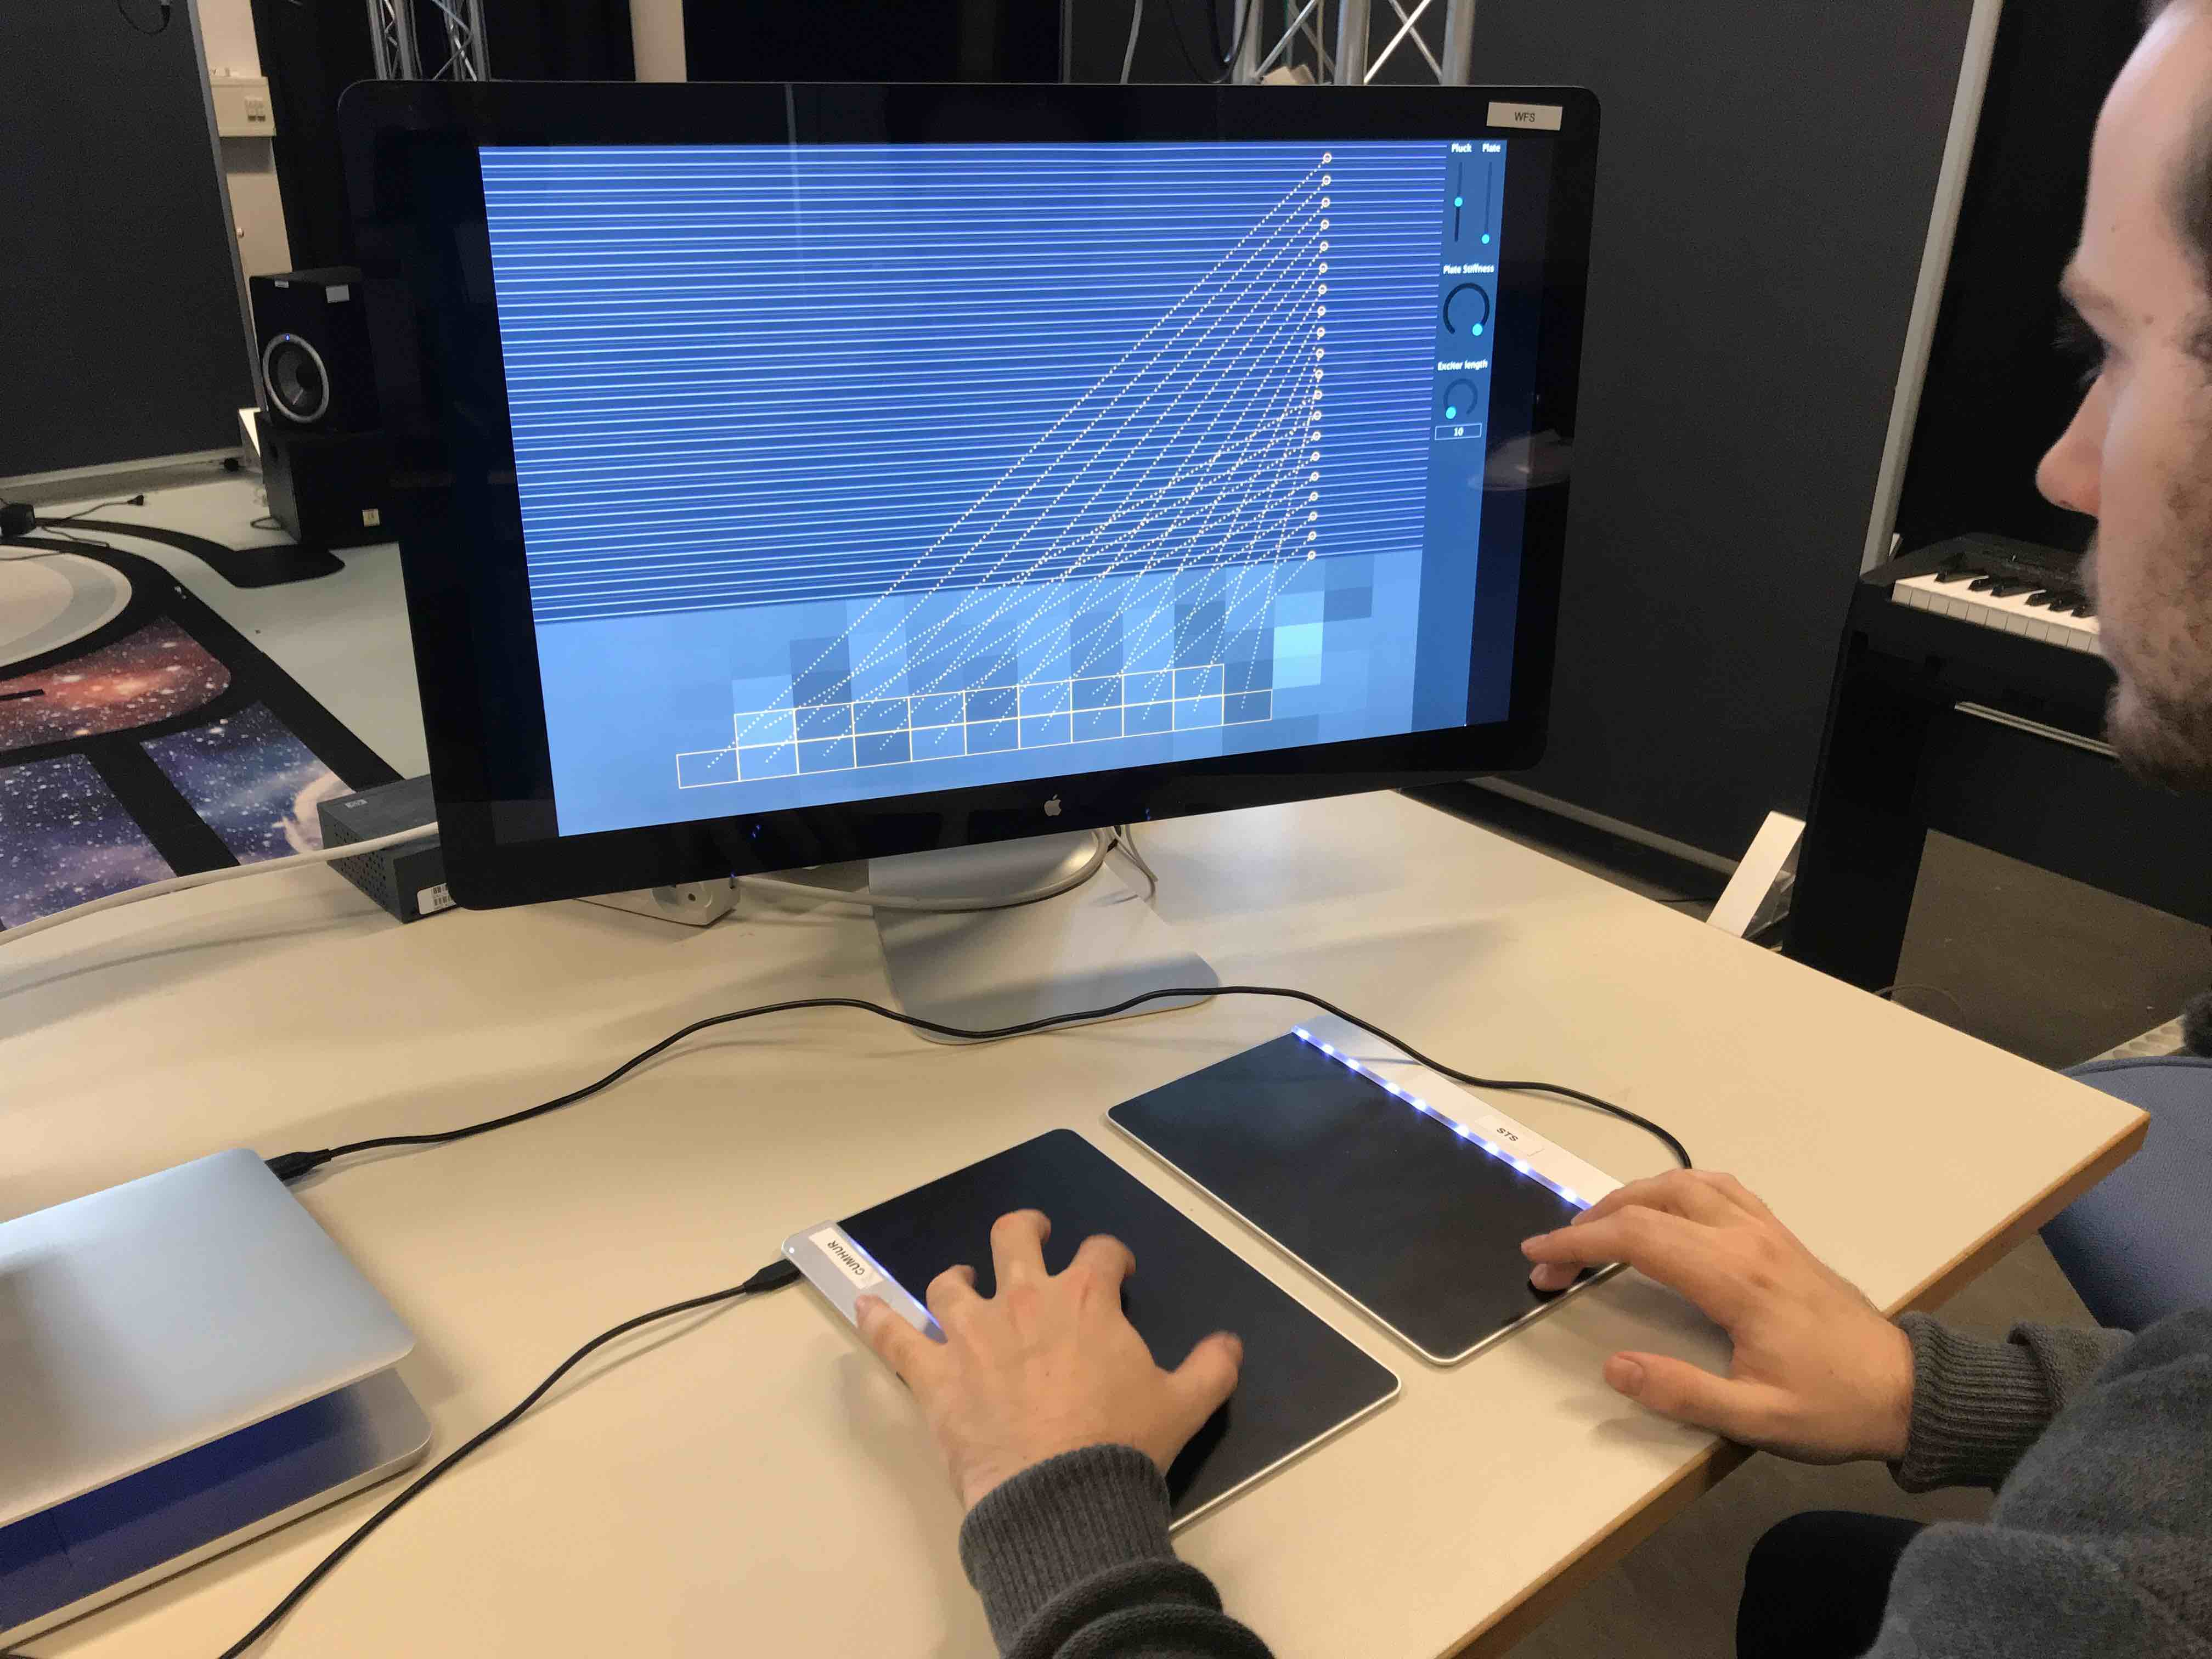
\includegraphics[width=1.0\columnwidth]{senselLQ.jpg}\centering
\caption{Player using the Sensel Morphs to interact with one of the instruments.\label{fig:sensel}}
\end{figure}

Strings are shown as coloured paths (see Figure \ref{fig:bowedSitar} for a descriptive visualisation). The state of the string is visualised using the vertical displacement of the paths. Bowed strings are shown in cyan on the top left. The bow is shown as a yellow rectangle and moves while interacting.
The fretting position is shown as a yellow circle. Plucked strings are shown in purple in the top right, underneath which the sympathetic strings are shown in light green. The plate is shown in the bottom using a grid of rectangles (clamped grid points are not shown). Its state is visualised using a grey-scale. Furthermore, connections are shown using orange circles/squares for the points of connection and dotted lines between these points. Lastly, all parameters that are controlled by the mouse such as output-level and plate-stiffness are located in a column on the right side of the application.

\section{Implemented Instruments}
We subdivide string-elements into three types: bowed, plucked and sympathetic strings. All strings will be connected to one plate acting as an instrument body of which the user can control the plate-stiffness. Furthermore, the user can change the output-level of each element type. Apart from these parameters, which are controlled by the mouse, the instruments are fully controlled by two Sensels. The instruments we have chosen as our inspiration are the sitar, the hammered dulcimer and the hurdy gurdy.

\subsection{Bowed Sitar}
The sitar is originally an Indian string instrument that has both fretted strings and sympathetic strings. Instead of plucking the fretted strings, we extended the model to bow them. Our implementation consists of 2 bowed strings (tuned to A3 and E4), 13 sympathetic strings (tuned according to \cite{sitarTuning}) and 5 plucked strings (tuned A3-E4 following an A-major scale) as it is also possible to strum the sympathetic strings. Figure \ref{fig:bowedSitar} shows the visual interface of the implementation. One Sensel is vertically subdivided into two sections; one for each bowed string. The first finger registered by the Sensel is mapped to a bow and the second is mapped to a fretting finger controlling pitch. The horizontal position of both fingers is visualised using the Sensel's LED array. The frets are not implemented as such (the pitch is continuous), but they are visualised for reference. 


\begin{figure*}[h]
\centering
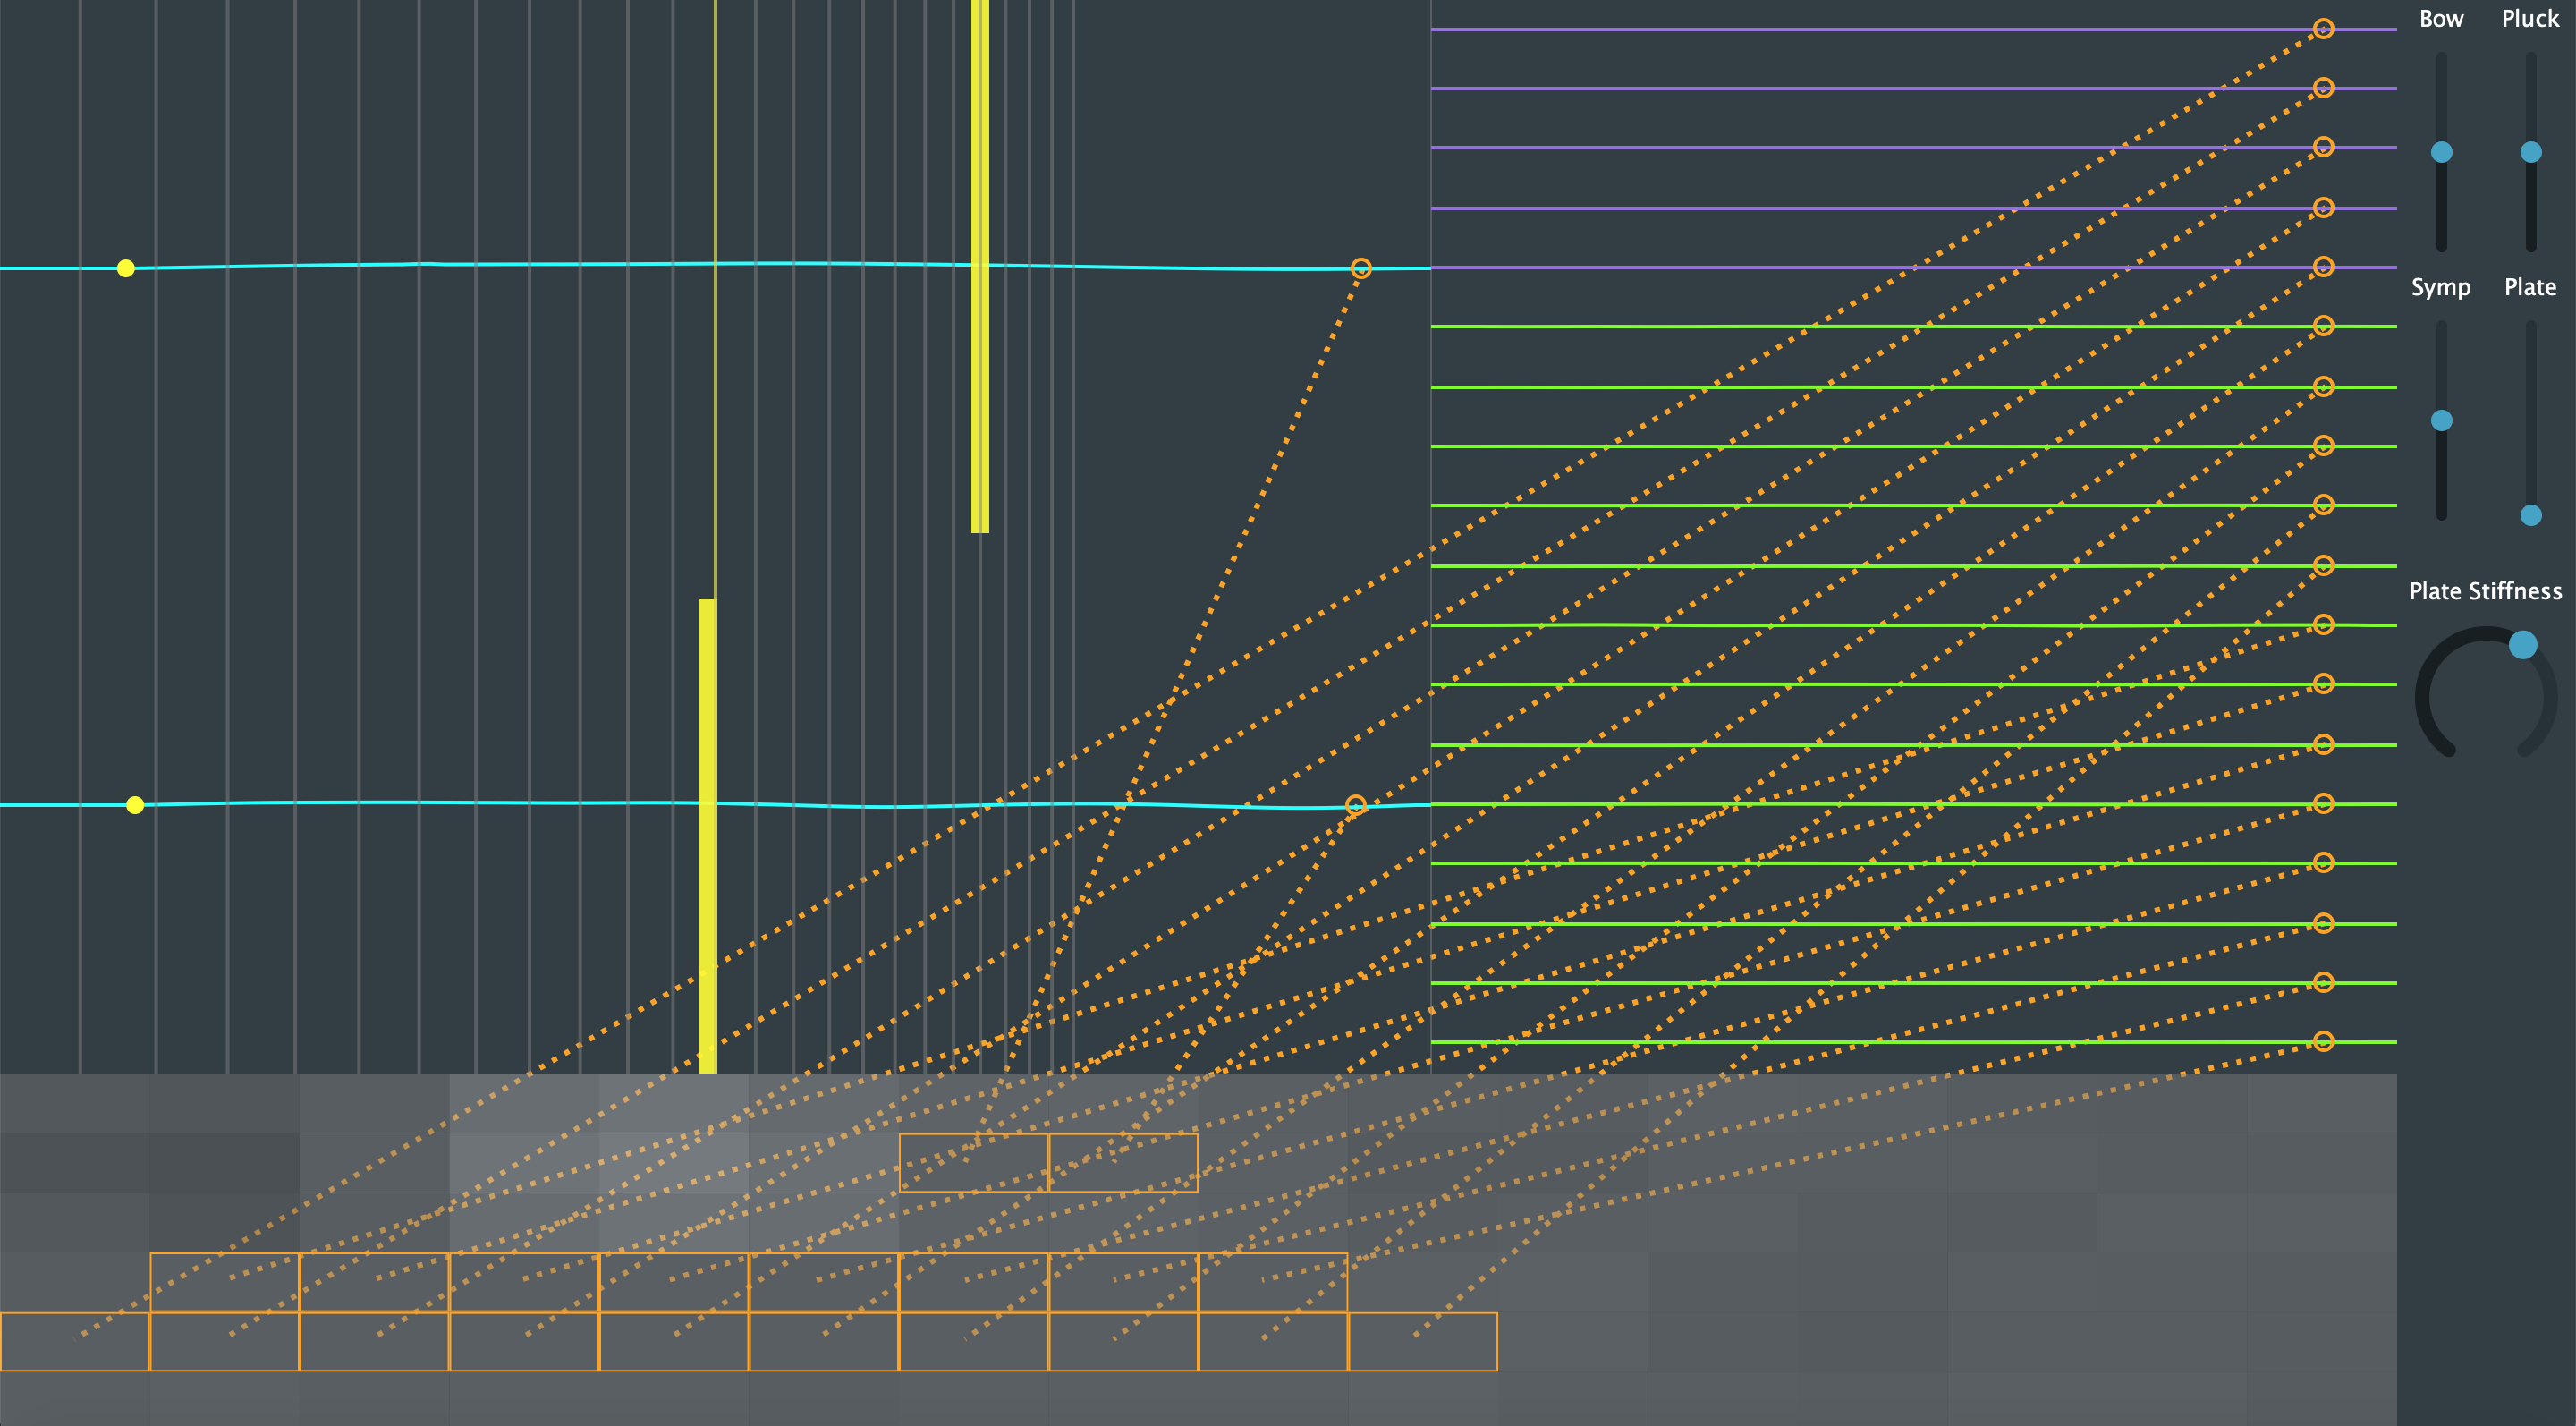
\includegraphics[width=1.5\columnwidth]{BowedSitar.png}
\caption{The bowed sitar application. The descriptions of the different elements and other objects are shown in the image, but will (naturally) not be visible in the application. \label{fig:bowedSitar}}
\end{figure*}

\subsection{Hammered Dulcimer}
The hammered dulcimer is an instrument that can be seen as an `open piano' where the musician has the hammers in their hand. Just like the piano, the strings are grouped in pairs or triplets
that are played simultaneously. 
The interface for the hammered dulcimer can be seen in Figure  \ref{fig:dulcimer}.
In our implementation, we have 20 pairs of plucked strings. Even though most hammered dulcimers have more strings, we decided that this configuration has the highest number of strings while maintaining playability. One of each pair is connected to a plate which slightly detunes it, creating a desired `chorusing' effect. 
Two Sensel boards are placed vertically next to each other (see Figure \ref{fig:sensel}). The pair with the lowest frequency is located in the bottom right and the highest in the top left, as in the real instrument. As with the plucked strings of the bowed sitar, the LED array is used to visualise the way that the Sensel is subdivided, which is especially useful here as one Sensel controls 10 string-pairs. 

The mass ratio is set relatively high ($\mathcal{M} = 100$) to amplify the non-linear interaction between the strings and the detuning of the strings connected to the plate. 

\begin{figure}[h]
\centering
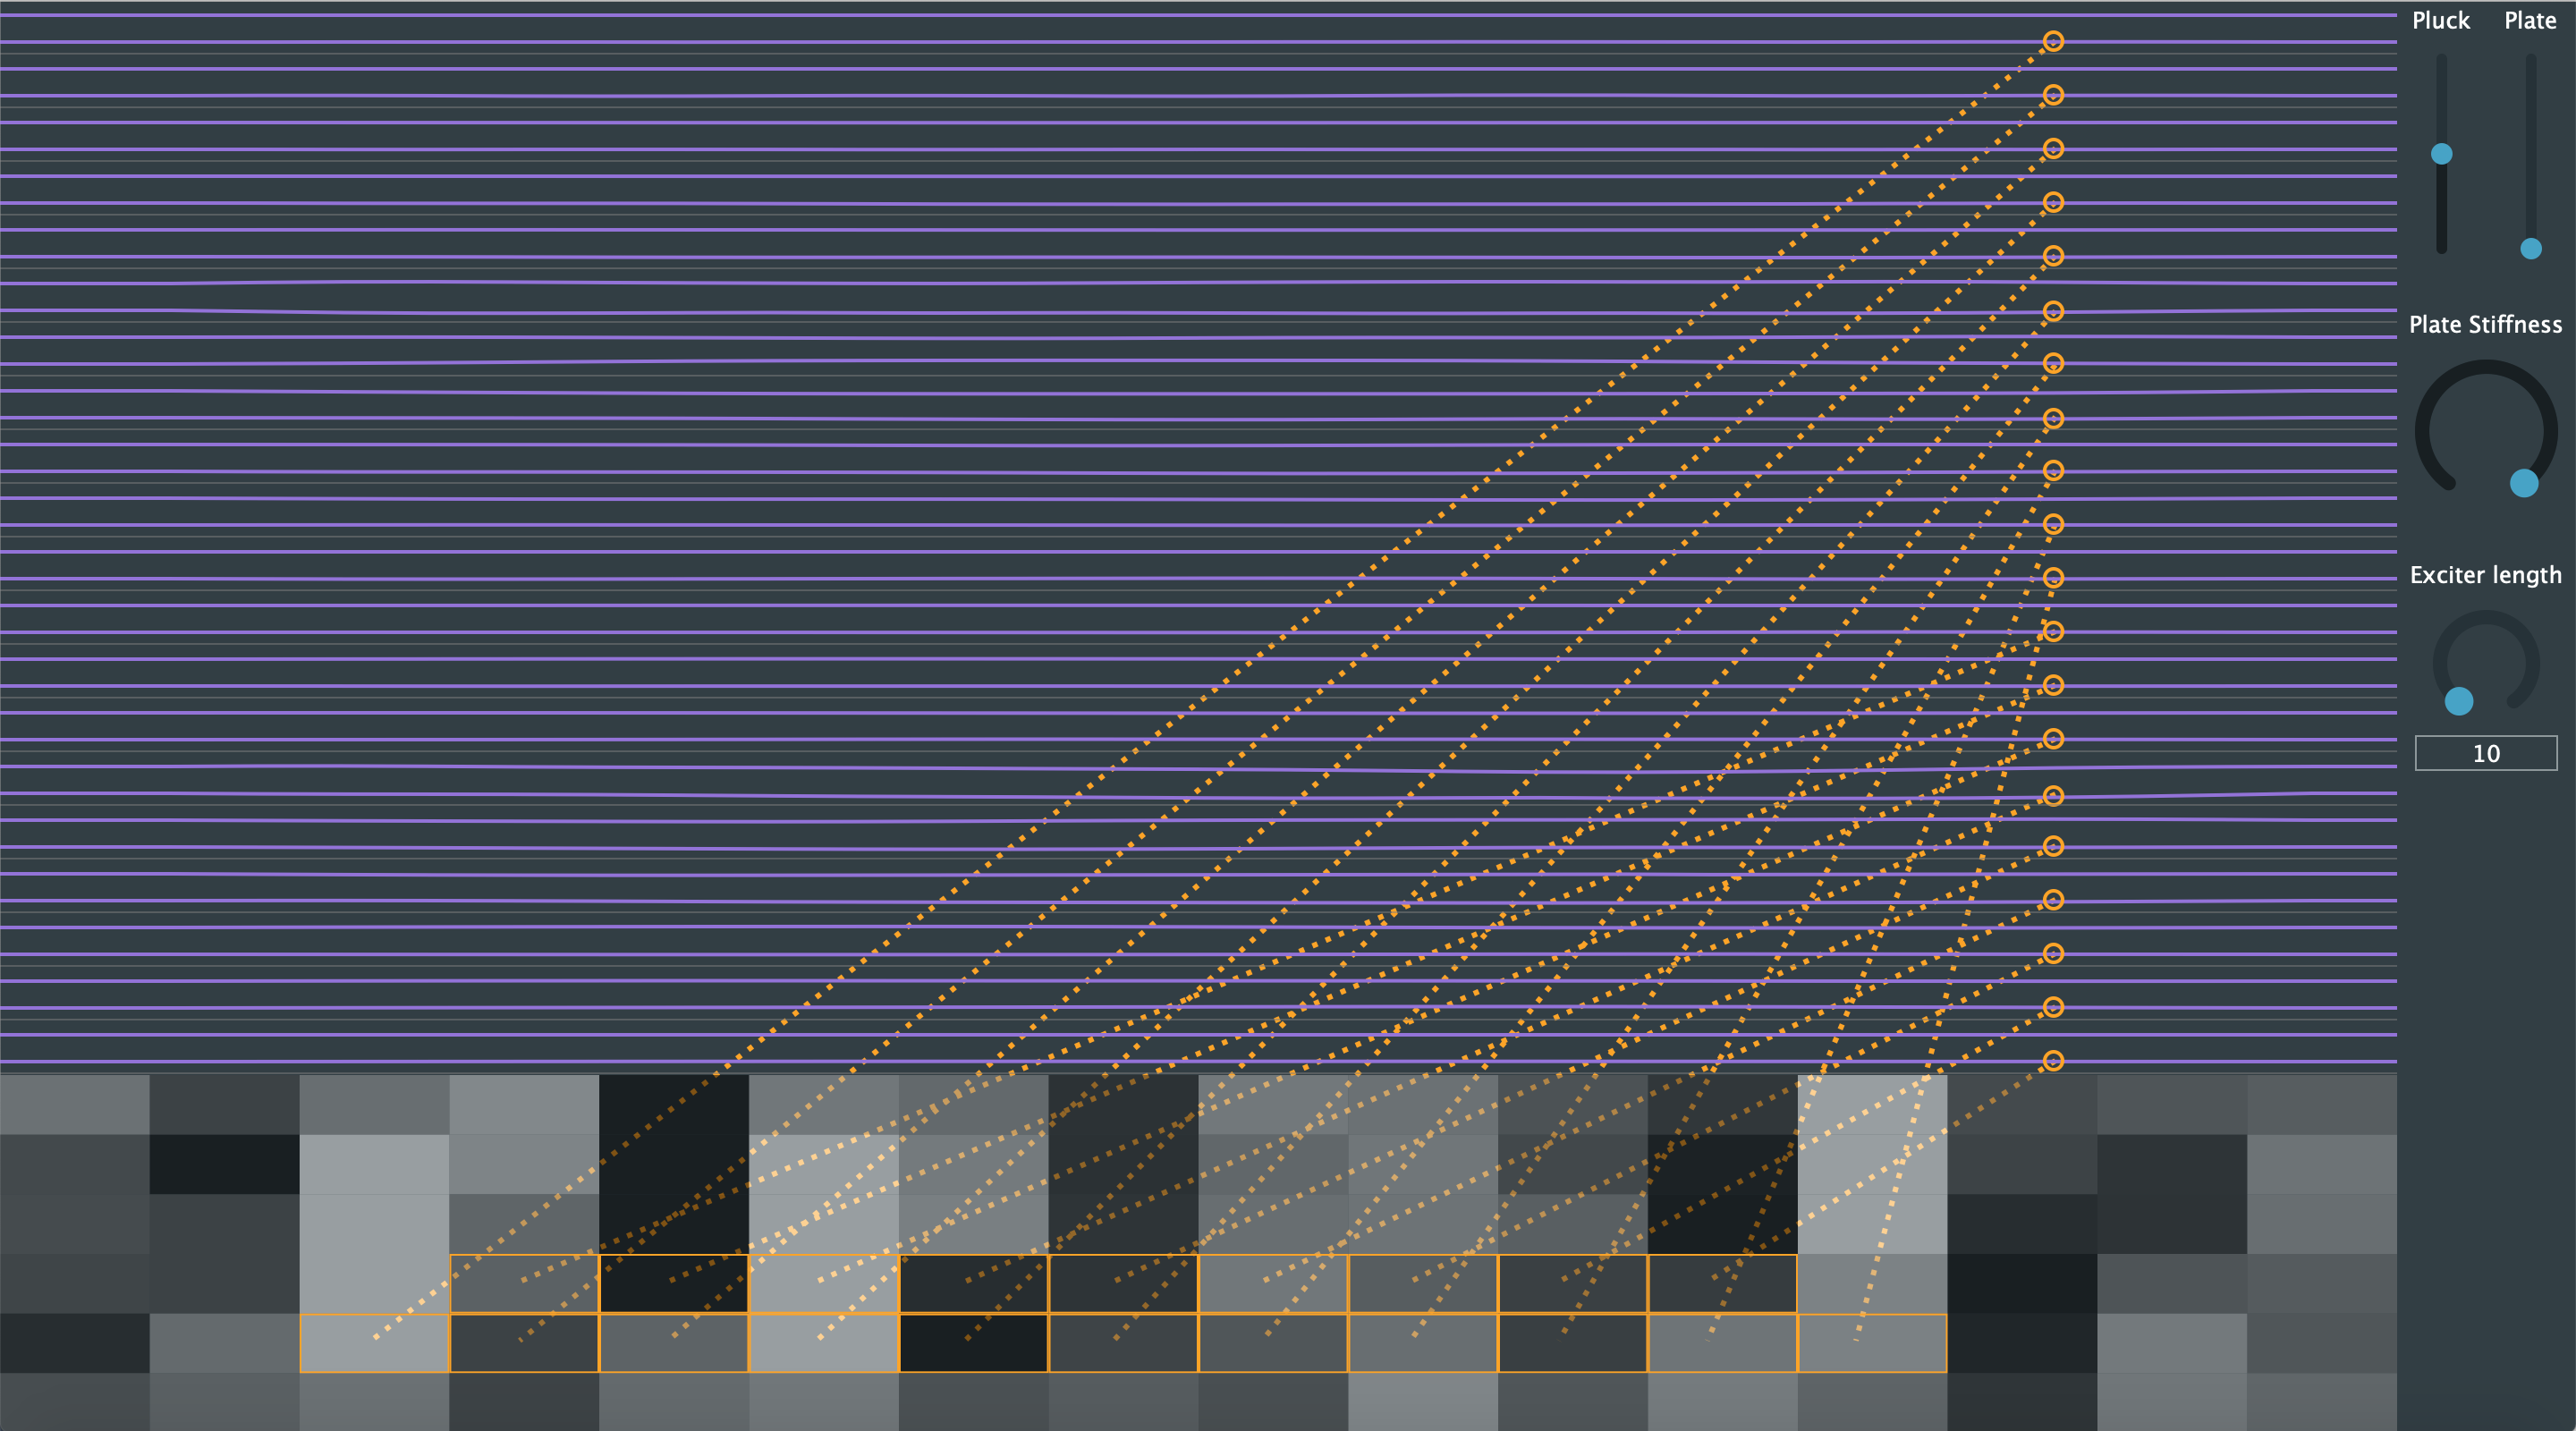
\includegraphics[width=1.0\columnwidth]{dulcimer.png}
\caption{The hammered dulcimer application. \label{fig:dulcimer}}
\end{figure}

\subsection{Hurdy Gurdy}
The hurdy gurdy is an instrument that consists of bowed and sympathetic strings. The bowing happens through a rosined wheel attached to a crank and bows these strings as the crank is turned. It is possible to change the pitch of a few bowed strings - the melody strings - using buttons that press tangent pins on the strings at different positions. The other strings, referred to as drone strings, are mostly tuned lower than the melody strings and provide the bass frequencies of the instrument. The musician can place the bowed strings on rests that keep the wheel from interacting with it. 
The visual interface can be seen in Figure \ref{fig:hurdyGurdy}.
Our implementation consists of 5 bowed strings subdivided into 2 drone strings tuned to A2, E3 and 3 melody strings tuned to A3, E4 and A4 and 13 sympathetic strings tuned the same way as the sympathetic strings in bowed sitar. Furthermore, the mass ratios have been set the same as in the bowed sitar application.

The Sensel is vertically subdivided into 5 rows that control whether the strings are placed on the wheel. 

\begin{figure}[h]
\centering
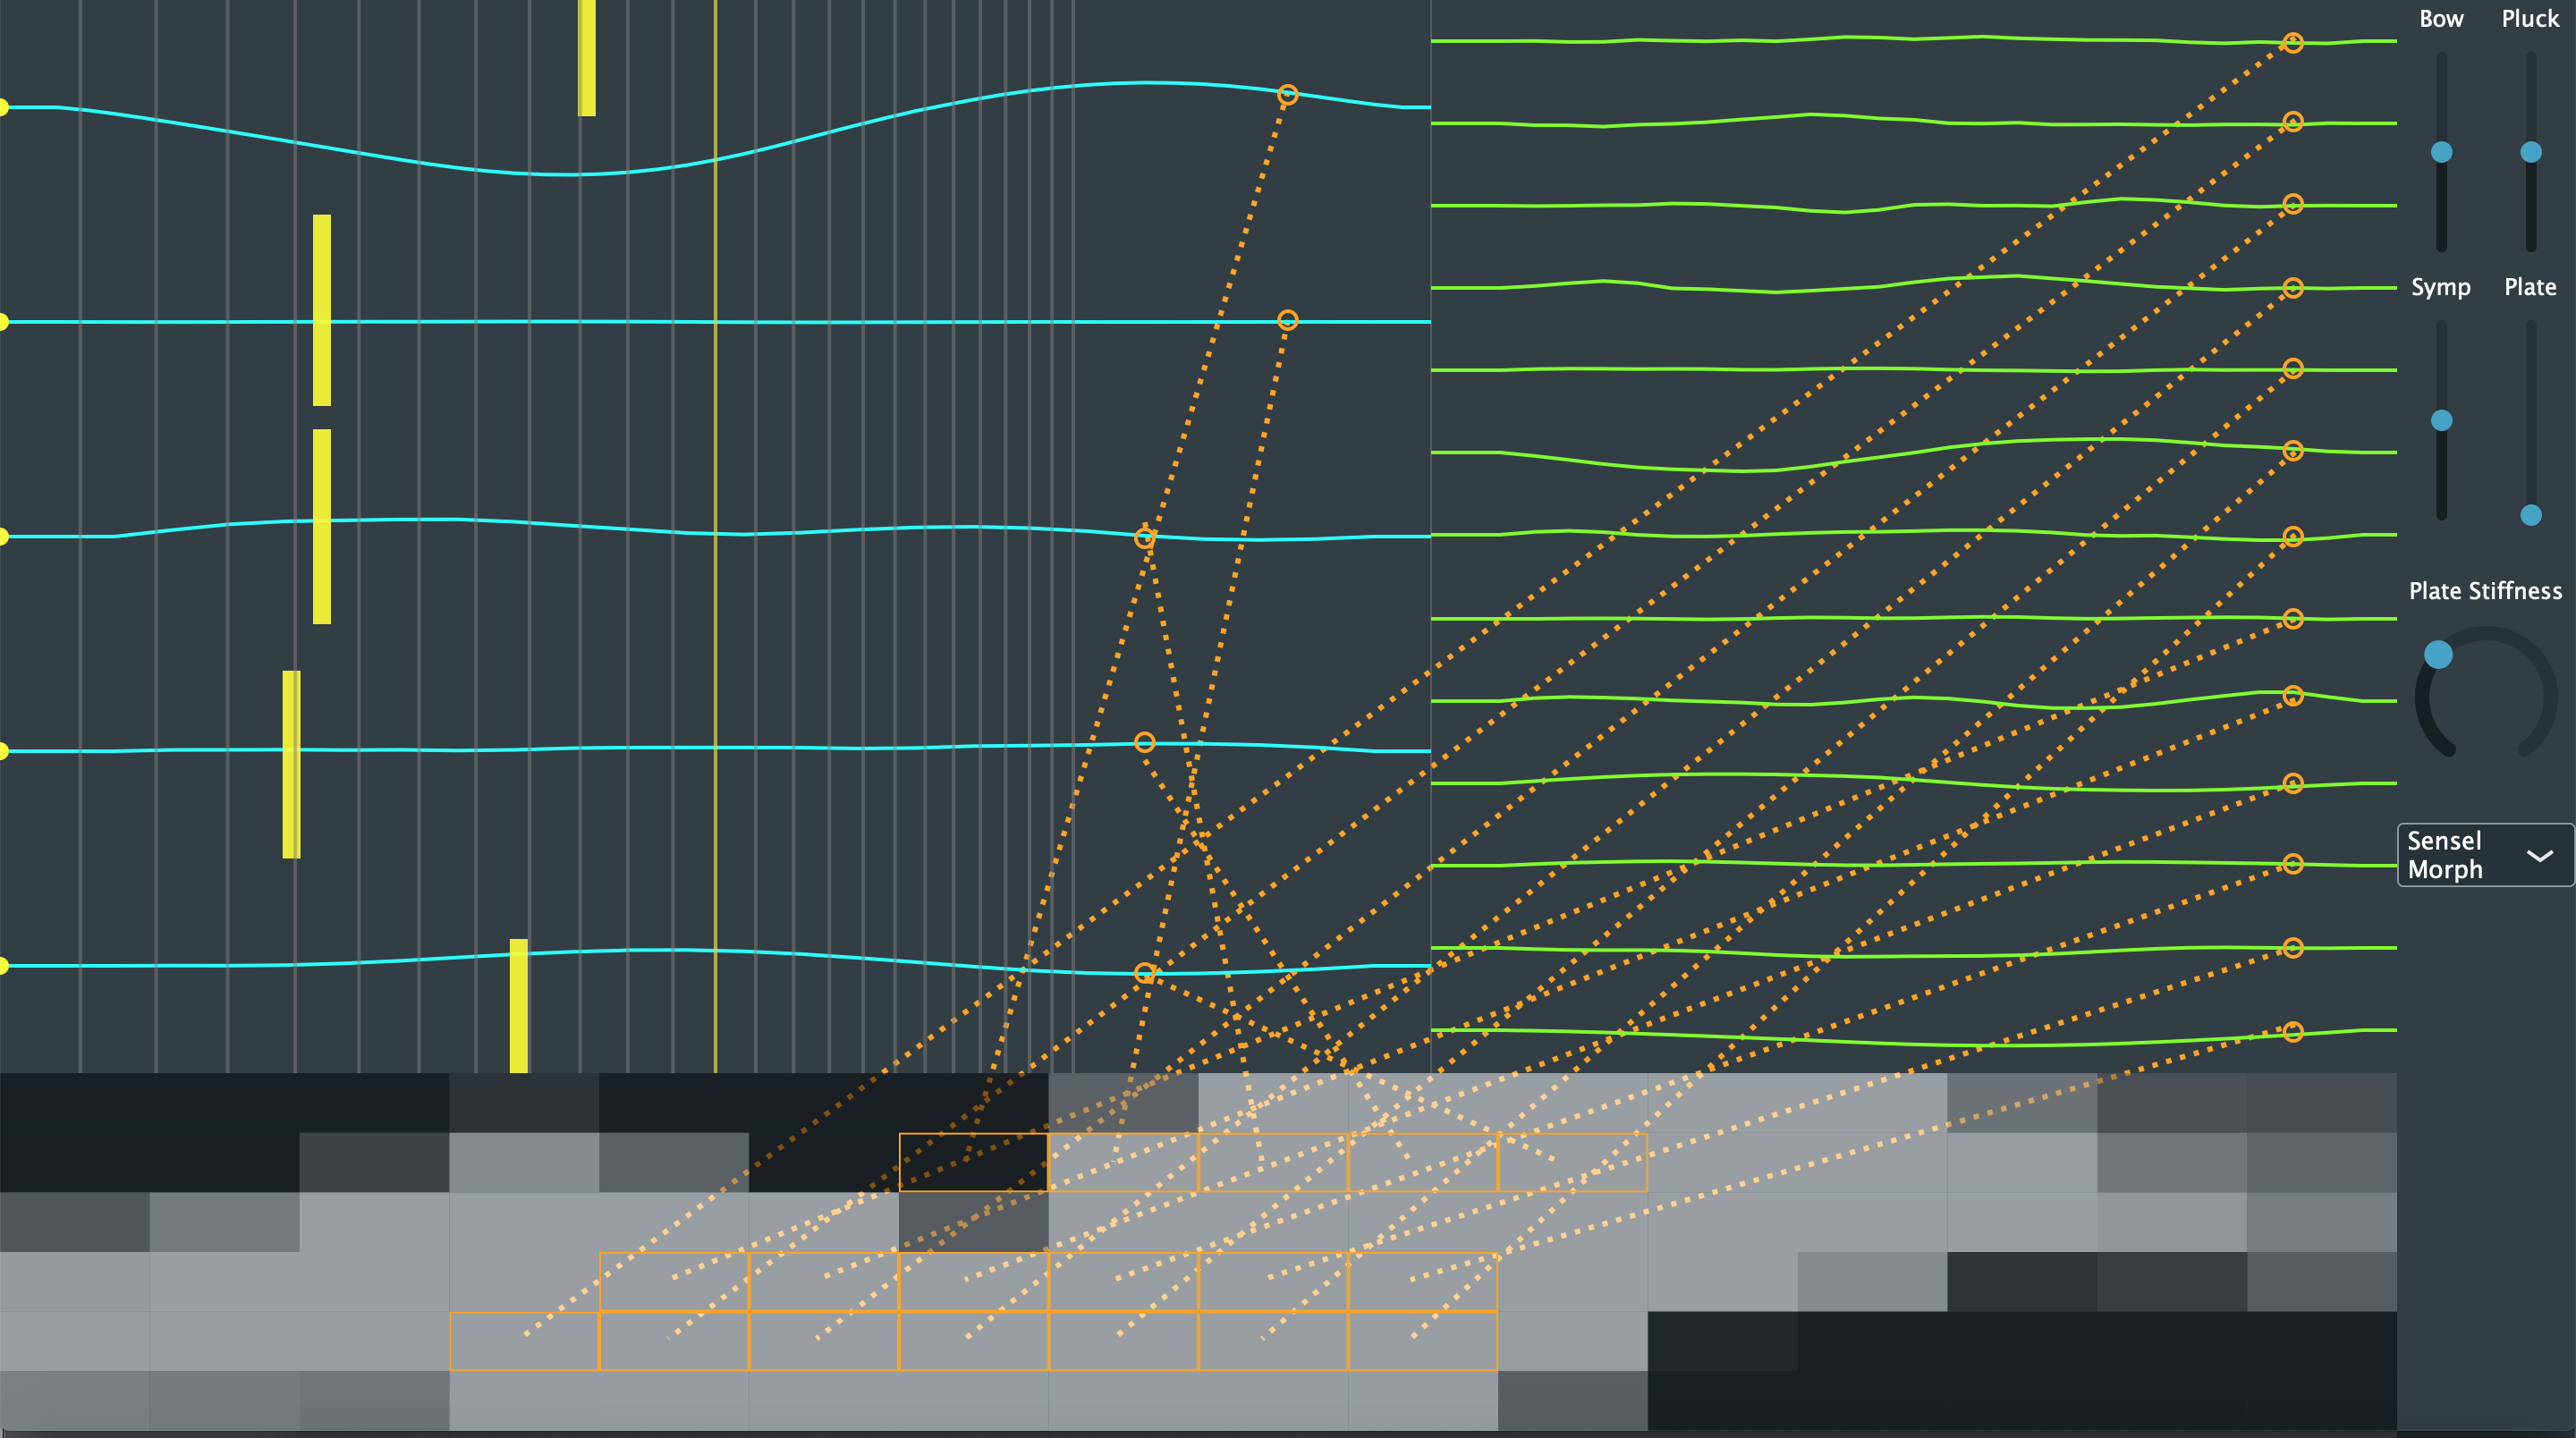
\includegraphics[width=1.0\columnwidth]{HurdyGurdy.png}
\caption{The hurdy gurdy application. \label{fig:hurdyGurdy}}
\end{figure}

\bibliography{smc2019bib}

\end{document}
